%% bare_jrnl.tex
%% V1.4b
%% 2015/08/26
%% by Michael Shell
%% see http://www.michaelshell.org/
%% for current contact information.
%%
%% This is a skeleton file demonstrating the use of IEEEtran.cls
%% (requires IEEEtran.cls version 1.8b or later) with an IEEE
%% journal paper.
%%
%% Support sites:
%% http://www.michaelshell.org/tex/ieeetran/
%% http://www.ctan.org/pkg/ieeetran
%% and
%% http://www.ieee.org/

%%*************************************************************************
%% Legal Notice:
%% This code is offered as-is without any warranty either expressed or
%% implied; without even the implied warranty of MERCHANTABILITY or
%% FITNESS FOR A PARTICULAR PURPOSE! 
%% User assumes all risk.
%% In no event shall the IEEE or any contributor to this code be liable for
%% any damages or losses, including, but not limited to, incidental,
%% consequential, or any other damages, resulting from the use or misuse
%% of any information contained here.
%%
%% All comments are the opinions of their respective authors and are not
%% necessarily endorsed by the IEEE.
%%
%% This work is distributed under the LaTeX Project Public License (LPPL)
%% ( http://www.latex-project.org/ ) version 1.3, and may be freely used,
%% distributed and modified. A copy of the LPPL, version 1.3, is included
%% in the base LaTeX documentation of all distributions of LaTeX released
%% 2003/12/01 or later.
%% Retain all contribution notices and credits.
%% ** Modified files should be clearly indicated as such, including  **
%% ** renaming them and changing author support contact information. **
%%*************************************************************************


% *** Authors should verify (and, if needed, correct) their LaTeX system  ***
% *** with the testflow diagnostic prior to trusting their LaTeX platform ***
% *** with production work. The IEEE's font choices and paper sizes can   ***
% *** trigger bugs that do not appear when using other class files.       ***                          ***
% The testflow support page is at:
% http://www.michaelshell.org/tex/testflow/



\documentclass[journal]{IEEEtran}
%
% If IEEEtran.cls has not been installed into the LaTeX system files,
% manually specify the path to it like:
% \documentclass[journal]{../sty/IEEEtran}





% Some very useful LaTeX packages include:
% (uncomment the ones you want to load)


% *** MISC UTILITY PACKAGES ***
%
%\usepackage{ifpdf}
% Heiko Oberdiek's ifpdf.sty is very useful if you need conditional
% compilation based on whether the output is pdf or dvi.
% usage:
% \ifpdf
%   % pdf code
% \else
%   % dvi code
% \fi
% The latest version of ifpdf.sty can be obtained from:
% http://www.ctan.org/pkg/ifpdf
% Also, note that IEEEtran.cls V1.7 and later provides a builtin
% \ifCLASSINFOpdf conditional that works the same way.
% When switching from latex to pdflatex and vice-versa, the compiler may
% have to be run twice to clear warning/error messages.






% *** CITATION PACKAGES ***
%
%\usepackage{cite}
% cite.sty was written by Donald Arseneau
% V1.6 and later of IEEEtran pre-defines the format of the cite.sty package
% \cite{} output to follow that of the IEEE. Loading the cite package will
% result in citation numbers being automatically sorted and properly
% "compressed/ranged". e.g., [1], [9], [2], [7], [5], [6] without using
% cite.sty will become [1], [2], [5]--[7], [9] using cite.sty. cite.sty's
% \cite will automatically add leading space, if needed. Use cite.sty's
% noadjust option (cite.sty V3.8 and later) if you want to turn this off
% such as if a citation ever needs to be enclosed in parenthesis.
% cite.sty is already installed on most LaTeX systems. Be sure and use
% version 5.0 (2009-03-20) and later if using hyperref.sty.
% The latest version can be obtained at:
% http://www.ctan.org/pkg/cite
% The documentation is contained in the cite.sty file itself.






% *** GRAPHICS RELATED PACKAGES ***
%
\ifCLASSINFOpdf
   \usepackage[pdftex]{graphicx}
  % declare the path(s) where your graphic files are
  % \graphicspath{{../pdf/}{../jpeg/}}
  % and their extensions so you won't have to specify these with
  % every instance of \includegraphics
  % \DeclareGraphicsExtensions{.pdf,.jpeg,.png}
\else
  % or other class option (dvipsone, dvipdf, if not using dvips). graphicx
  % will default to the driver specified in the system graphics.cfg if no
  % driver is specified.
  % \usepackage[dvips]{graphicx}
  % declare the path(s) where your graphic files are
  % \graphicspath{{../eps/}}
  % and their extensions so you won't have to specify these with
  % every instance of \includegraphics
  % \DeclareGraphicsExtensions{.eps}
\fi
% graphicx was written by David Carlisle and Sebastian Rahtz. It is
% required if you want graphics, photos, etc. graphicx.sty is already
% installed on most LaTeX systems. The latest version and documentation
% can be obtained at: 
% http://www.ctan.org/pkg/graphicx
% Another good source of documentation is "Using Imported Graphics in
% LaTeX2e" by Keith Reckdahl which can be found at:
% http://www.ctan.org/pkg/epslatex
%
% latex, and pdflatex in dvi mode, support graphics in encapsulated
% postscript (.eps) format. pdflatex in pdf mode supports graphics
% in .pdf, .jpeg, .png and .mps (metapost) formats. Users should ensure
% that all non-photo figures use a vector format (.eps, .pdf, .mps) and
% not a bitmapped formats (.jpeg, .png). The IEEE frowns on bitmapped formats
% which can result in "jaggedy"/blurry rendering of lines and letters as
% well as large increases in file sizes.
%
% You can find documentation about the pdfTeX application at:
% http://www.tug.org/applications/pdftex





% *** MATH PACKAGES ***
%
% \usepackage{amsmath}
% A popular package from the American Mathematical Society that provides
% many useful and powerful commands for dealing with mathematics.
%
% Note that the amsmath package sets \interdisplaylinepenalty to 10000
% thus preventing page breaks from occurring within multiline equations. Use:
%\interdisplaylinepenalty=2500
% after loading amsmath to restore such page breaks as IEEEtran.cls normally
% does. amsmath.sty is already installed on most LaTeX systems. The latest
% version and documentation can be obtained at:
% http://www.ctan.org/pkg/amsmath





% *** SPECIALIZED LIST PACKAGES ***
%
\usepackage{algorithmic}
% algorithmic.sty was written by Peter Williams and Rogerio Brito.
% This package provides an algorithmic environment fo describing algorithms.
% You can use the algorithmic environment in-text or within a figure
% environment to provide for a floating algorithm. Do NOT use the algorithm
% floating environment provided by algorithm.sty (by the same authors) or
% algorithm2e.sty (by Christophe Fiorio) as the IEEE does not use dedicated
% algorithm float types and packages that provide these will not provide
% correct IEEE style captions. The latest version and documentation of
% algorithmic.sty can be obtained at:
% http://www.ctan.org/pkg/algorithms
% Also of interest may be the (relatively newer and more customizable)
% algorithmicx.sty package by Szasz Janos:
% http://www.ctan.org/pkg/algorithmicx




% *** ALIGNMENT PACKAGES ***
%
\usepackage{array}
% Frank Mittelbach's and David Carlisle's array.sty patches and improves
% the standard LaTeX2e array and tabular environments to provide better
% appearance and additional user controls. As the default LaTeX2e table
% generation code is lacking to the point of almost being broken with
% respect to the quality of the end results, all users are strongly
% advised to use an enhanced (at the very least that provided by array.sty)
% set of table tools. array.sty is already installed on most systems. The
% latest version and documentation can be obtained at:
% http://www.ctan.org/pkg/array


% IEEEtran contains the IEEEeqnarray family of commands that can be used to
% generate multiline equations as well as matrices, tables, etc., of high
% quality.




% *** SUBFIGURE PACKAGES ***
\ifCLASSOPTIONcompsoc
  \usepackage[caption=false,font=normalsize,labelfont=sf,textfont=sf]{subfig}
\else
  \usepackage[caption=false,font=footnotesize]{subfig}
\fi
% subfig.sty, written by Steven Douglas Cochran, is the modern replacement
% for subfigure.sty, the latter of which is no longer maintained and is
% incompatible with some LaTeX packages including fixltx2e. However,
% subfig.sty requires and automatically loads Axel Sommerfeldt's caption.sty
% which will override IEEEtran.cls' handling of captions and this will result
% in non-IEEE style figure/table captions. To prevent this problem, be sure
% and invoke subfig.sty's "caption=false" package option (available since
% subfig.sty version 1.3, 2005/06/28) as this is will preserve IEEEtran.cls
% handling of captions.
% Note that the Computer Society format requires a larger sans serif font
% than the serif footnote size font used in traditional IEEE formatting
% and thus the need to invoke different subfig.sty package options depending
% on whether compsoc mode has been enabled.
%
% The latest version and documentation of subfig.sty can be obtained at:
% http://www.ctan.org/pkg/subfig




% *** FLOAT PACKAGES ***
%
\usepackage{fixltx2e}
% fixltx2e, the successor to the earlier fix2col.sty, was written by
% Frank Mittelbach and David Carlisle. This package corrects a few problems
% in the LaTeX2e kernel, the most notable of which is that in current
% LaTeX2e releases, the ordering of single and double column floats is not
% guaranteed to be preserved. Thus, an unpatched LaTeX2e can allow a
% single column figure to be placed prior to an earlier double column
% figure.
% Be aware that LaTeX2e kernels dated 2015 and later have fixltx2e.sty's
% corrections already built into the system in which case a warning will
% be issued if an attempt is made to load fixltx2e.sty as it is no longer
% needed.
% The latest version and documentation can be found at:
% http://www.ctan.org/pkg/fixltx2e


%\usepackage{stfloats}
% stfloats.sty was written by Sigitas Tolusis. This package gives LaTeX2e
% the ability to do double column floats at the bottom of the page as well
% as the top. (e.g., "\begin{figure*}[!b]" is not normally possible in
% LaTeX2e). It also provides a command:
%\fnbelowfloat
% to enable the placement of footnotes below bottom floats (the standard
% LaTeX2e kernel puts them above bottom floats). This is an invasive package
% which rewrites many portions of the LaTeX2e float routines. It may not work
% with other packages that modify the LaTeX2e float routines. The latest
% version and documentation can be obtained at:
% http://www.ctan.org/pkg/stfloats
% Do not use the stfloats baselinefloat ability as the IEEE does not allow
% \baselineskip to stretch. Authors submitting work to the IEEE should note
% that the IEEE rarely uses double column equations and that authors should try
% to avoid such use. Do not be tempted to use the cuted.sty or midfloat.sty
% packages (also by Sigitas Tolusis) as the IEEE does not format its papers in
% such ways.
% Do not attempt to use stfloats with fixltx2e as they are incompatible.
% Instead, use Morten Hogholm'a dblfloatfix which combines the features
% of both fixltx2e and stfloats:
%
% \usepackage{dblfloatfix}
% The latest version can be found at:
% http://www.ctan.org/pkg/dblfloatfix




%\ifCLASSOPTIONcaptionsoff
%  \usepackage[nomarkers]{endfloat}
% \let\MYoriglatexcaption\caption
% \renewcommand{\caption}[2][\relax]{\MYoriglatexcaption[#2]{#2}}
%\fi
% endfloat.sty was written by James Darrell McCauley, Jeff Goldberg and 
% Axel Sommerfeldt. This package may be useful when used in conjunction with 
% IEEEtran.cls'  captionsoff option. Some IEEE journals/societies require that
% submissions have lists of figures/tables at the end of the paper and that
% figures/tables without any captions are placed on a page by themselves at
% the end of the document. If needed, the draftcls IEEEtran class option or
% \CLASSINPUTbaselinestretch interface can be used to increase the line
% spacing as well. Be sure and use the nomarkers option of endfloat to
% prevent endfloat from "marking" where the figures would have been placed
% in the text. The two hack lines of code above are a slight modification of
% that suggested by in the endfloat docs (section 8.4.1) to ensure that
% the full captions always appear in the list of figures/tables - even if
% the user used the short optional argument of \caption[]{}.
% IEEE papers do not typically make use of \caption[]'s optional argument,
% so this should not be an issue. A similar trick can be used to disable
% captions of packages such as subfig.sty that lack options to turn off
% the subcaptions:
% For subfig.sty:
% \let\MYorigsubfloat\subfloat
% \renewcommand{\subfloat}[2][\relax]{\MYorigsubfloat[]{#2}}
% However, the above trick will not work if both optional arguments of
% the \subfloat command are used. Furthermore, there needs to be a
% description of each subfigure *somewhere* and endfloat does not add
% subfigure captions to its list of figures. Thus, the best approach is to
% avoid the use of subfigure captions (many IEEE journals avoid them anyway)
% and instead reference/explain all the subfigures within the main caption.
% The latest version of endfloat.sty and its documentation can obtained at:
% http://www.ctan.org/pkg/endfloat
%
% The IEEEtran \ifCLASSOPTIONcaptionsoff conditional can also be used
% later in the document, say, to conditionally put the References on a 
% page by themselves.




% *** PDF, URL AND HYPERLINK PACKAGES ***
%
\usepackage{url}
% url.sty was written by Donald Arseneau. It provides better support for
% handling and breaking URLs. url.sty is already installed on most LaTeX
% systems. The latest version and documentation can be obtained at:
% http://www.ctan.org/pkg/url
% Basically, \url{my_url_here}.




% *** Do not adjust lengths that control margins, column widths, etc. ***
% *** Do not use packages that alter fonts (such as pslatex).         ***
% There should be no need to do such things with IEEEtran.cls V1.6 and later.
% (Unless specifically asked to do so by the journal or conference you plan
% to submit to, of course. )

%DIDI FIXES START:
\usepackage[T1]{fontenc}
\usepackage[utf8]{inputenc}
\usepackage[english]{babel}

\usepackage{aas_macros}

\usepackage{varioref}
\usepackage[english]{fancyref}  %better cross reference support
\usepackage[locale=UK,          %numbers and si unit translation
binary-units=true]{siunitx}     %enable binary units!
\sisetup{detect-weight=true, detect-family=true} %format like surrounding environment
\usepackage[autostyle=true]     %enquote and translation of quote style (en/de)
{csquotes}

\addto\captionsenglish{\renewcommand\figurename{Fig.}}
  
%extending fancyref for listings in both languages:
\newcommand*{\fancyreflstlabelprefix}{lst}
\fancyrefaddcaptions{english}{%
  \providecommand*{\freflstname}{listing}%
  \providecommand*{\Freflstname}{Listing}%
}
\fancyrefaddcaptions{german}{%
  \providecommand*{\freflstname}{Listing}%
  \providecommand*{\Freflstname}{Listing}%
}
\frefformat{plain}{\fancyreflstlabelprefix}{\freflstname\fancyrefdefaultspacing#1}
\Frefformat{plain}{\fancyreflstlabelprefix}{\Freflstname\fancyrefdefaultspacing#1}
\frefformat{vario}{\fancyreflstlabelprefix}{%
  \freflstname\fancyrefdefaultspacing#1#3%
}
\Frefformat{vario}{\fancyreflstlabelprefix}{%
  \Freflstname\fancyrefdefaultspacing#1#3%
}
%extend fancyref for my own figure text:
\newcommand*{\fancyrefmyfiglabelprefix}{myfig}
\fancyrefaddcaptions{english}{%
  \providecommand*{\frefmyfigname}{Fig.}%
  \providecommand*{\Frefmyfigname}{Fig.}%
}
\fancyrefaddcaptions{german}{%
  \providecommand*{\frefmyfigname}{Fig.}%
  \providecommand*{\Frefmyfigname}{Fig.}%
}
\frefformat{plain}{\fancyrefmyfiglabelprefix}{\frefmyfigname\fancyrefdefaultspacing#1}
\Frefformat{plain}{\fancyrefmyfiglabelprefix}{\Frefmyfigname\fancyrefdefaultspacing#1}
\frefformat{vario}{\fancyrefmyfiglabelprefix}{%
  \frefmyfigname\fancyrefdefaultspacing#1#3%
}
\Frefformat{vario}{\fancyrefmyfiglabelprefix}{%
  \Frefmyfigname\fancyrefdefaultspacing#1#3%
}
%extend fancyref for my own equation text (empty):
\newcommand*{\fancyrefmyeqlabelprefix}{myeq}
\fancyrefaddcaptions{english}{%
  \providecommand*{\frefmyeqname}{}%
  \providecommand*{\Frefmyeqname}{}%
}
\fancyrefaddcaptions{german}{%
  \providecommand*{\frefmyeqname}{}%
  \providecommand*{\Frefmyeqname}{}%
}
\frefformat{plain}{\fancyrefmyeqlabelprefix}{\frefmyeqname\fancyrefdefaultspacing\textup{(#1)}}
\Frefformat{plain}{\fancyrefmyeqlabelprefix}{\Frefmyeqname\fancyrefdefaultspacing\textup{(#1)}}
\frefformat{vario}{\fancyrefmyeqlabelprefix}{%
  \frefmyeqname\fancyrefdefaultspacing\textup{(#1)}#3%
}
\Frefformat{vario}{\fancyrefmyeqlabelprefix}{%
  \Frefmyeqname\fancyrefdefaultspacing\textup{(#1)}#3%
}

\usepackage{amsmath,amssymb,amstext,bm}% math packages
\usepackage{mathcomp}% symbols (perthousand, ...) in math mode

\usepackage{placeins} %\FloatBarrier

\usepackage[backend=biber,        %choose biber as literature reference backend
bibencoding=utf8,                 %.bib-File if utf8 encoded...
maxnames=5,                       %Max 5 authors, then et al.
minnames=1,                       %if et al., then only display first!
style=ieee
]{biblatex}
\bibliography{bib/literatur}      %literatur.bib will be loaded as literature file!

\usepackage[%
breaklinks=true,% allow line break in links
colorlinks=false,% if true: disables framed link on unprinted version
linkcolor=black,anchorcolor=black,citecolor=black,filecolor=black,%
menucolor=black,urlcolor=black,bookmarksnumbered=true]{hyperref}% hyperlinks for references

\setcounter{biburlnumpenalty}{100}%make URLs in bibliography breakable
\setcounter{biburlucpenalty}{100} %make URLs in bibliography breakable
\setcounter{biburllcpenalty}{100} %make URLs in bibliography breakable

\usepackage[acronym,nomain]{glossaries}%Abkürzungsverzeichnis ohne Glossar
%\newacronym{label}{Abkürz.}{Langvers.}
%\newacronym[shortplural=Abk.(Plural),longplural=Langvers.(Plural)]{label}{Abk.}{Langvers.}
\newacronym[shortplural=PCBs, longplural=printed circuit boards]{pcb}{PCB}{printed circuit board}
\newacronym[shortplural=ICs, longplural=integrated circuits]{ic}{IC}{integrated circuit}
\newacronym[shortplural=DSPs, longplural=digital signal processors]{dsp}{DSP}{digital signal processor}
\newacronym[shortplural=FIRs]{fir}{FIR}{finite impulse response}
\newacronym[shortplural=FFTs]{fft}{FFT}{fast Fourier transformation}
\newacronym[shortplural=KNNs]{knn}{KNN}{K-Nearest-Neighbour}
\newacronym[shortplural=GUIs]{gui}{GUI}{graphical user interface}
\newacronym{wisdm}{WISDM}{WIreless Sensor Data Mining}                  %Acronyme laden
\makeglossaries                   %Paket verwenden
%DIDI FIXES END


% correct bad hyphenation here
\hyphenation{op-tical net-works semi-conduc-tor}

\begin{document}
%
% paper title
% Titles are generally capitalized except for words such as a, an, and, as,
% at, but, by, for, in, nor, of, on, or, the, to and up, which are usually
% not capitalized unless they are the first or last word of the title.
% Linebreaks \\ can be used within to get better formatting as desired.
% Do not put math or special symbols in the title.
\title{Activity Recognition\\using KNN Classification and Transfer Learning}
%
%
% author names and IEEE memberships
% note positions of commas and nonbreaking spaces ( ~ ) LaTeX will not break
% a structure at a ~ so this keeps an author's name from being broken across
% two lines.
% use \thanks{} to gain access to the first footnote area
% a separate \thanks must be used for each paragraph as LaTeX2e's \thanks
% was not built to handle multiple paragraphs
%

\author{Dietmar Malli% <-this % stops a space
\thanks{Manuscript sent June 08, 2020; not yet revised.}}

% note the % following the last \IEEEmembership and also \thanks - 
% these prevent an unwanted space from occurring between the last author name
% and the end of the author line. i.e., if you had this:
% 
% \author{....lastname \thanks{...} \thanks{...} }
%                     ^------------^------------^----Do not want these spaces!
%
% a space would be appended to the last name and could cause every name on that
% line to be shifted left slightly. This is one of those "LaTeX things". For
% instance, "\textbf{A} \textbf{B}" will typeset as "A B" not "AB". To get
% "AB" then you have to do: "\textbf{A}\textbf{B}"
% \thanks is no different in this regard, so shield the last } of each \thanks
% that ends a line with a % and do not let a space in before the next \thanks.
% Spaces after \IEEEmembership other than the last one are OK (and needed) as
% you are supposed to have spaces between the names. For what it is worth,
% this is a minor point as most people would not even notice if the said evil
% space somehow managed to creep in.



% The paper headers
%\markboth{Article of WS 2017/18 442.181 Verfassen wissenschaftlicher Arbeiten: Equalizing a structure borne sound converter}
\markboth{Report of SS 2020 448.066 Mobile Computing Laboratory}%
{Activity Recognition using KNN Classification and Transfer Learning}
% The only time the second header will appear is for the odd numbered pages
% after the title page when using the twoside option.
% 
% *** Note that you probably will NOT want to include the author's ***
% *** name in the headers of peer review papers.                   ***
% You can use \ifCLASSOPTIONpeerreview for conditional compilation here if
% you desire.




% If you want to put a publisher's ID mark on the page you can do it like
% this:
%\IEEEpubid{0000--0000/00\$00.00~\copyright~2015 IEEE}
% Remember, if you use this you must call \IEEEpubidadjcol in the second
% column for its text to clear the IEEEpubid mark.



% use for special paper notices
%\IEEEspecialpapernotice{(Invited Paper)}




% make the title area
\maketitle

% As a general rule, do not put math, special symbols or citations
% in the abstract or keywords.
\begin{abstract}
This report describes the development of a mobile application which enables its users to track their activities using a \gls{knn} classifier as well as two machine learning based approaches. It also allows them to compare their performance immediately on device by providing graphs depicting the predictions of these algorithms.
\end{abstract}

% Note that keywords are not normally used for peerreview papers.
\begin{IEEEkeywords}
MCL, Mobile Computing Laboratory, TU Graz, Android, Transfer Learning, Activity Recognition, KNN Classification, Base Model, Head Model, Machine Learning
\end{IEEEkeywords}






% For peer review papers, you can put extra information on the cover
% page as needed:
% \ifCLASSOPTIONpeerreview
% \begin{center} \bfseries EDICS Category: 3-BBND \end{center}
% \fi
%
% For peerreview papers, this IEEEtran command inserts a page break and
% creates the second title. It will be ignored for other modes.
\IEEEpeerreviewmaketitle


% The very first letter is a 2 line initial drop letter followed
% by the rest of the first word in caps.
% 
% form to use if the first word consists of a single letter:
% \IEEEPARstart{A}{demo} file is ....
% 
% form to use if you need the single drop letter followed by
% normal text (unknown if ever used by the IEEE):
% \IEEEPARstart{A}{}demo file is ....
% 
% Some journals put the first two words in caps:
% \IEEEPARstart{T}{his demo} file is ....
% 
\section{Introduction}
\label{sec:intro}
\IEEEPARstart{T}{he} goal of this laboratory was to develop a mobile application which recognizes acitvities performed by the user of a smartphone. During the first part students were introduced to android as development platform as well as how sensors can be read on this platform. Further, a mobile application which recognizes a users activity based on the \gls{knn} algorithm had to be implemented. The decision which sensors to use, as well as which features to compute was also left open by the course organization. During the second part the \gls{knn} algorithm had to be compared to machine learning approaches. In detail a comparison to a completely pre-trained model, as well as a transfer-learning based model had to be done. This was done by extending the application from the first part of the laboratory.

Throughout the whole lecture it was tried to classify the same six categories of activity introduced by the \gls{wisdm} dataset\autocite{wisdm:dataset}:
\begin{itemize}
\item sitting
\item standing
\item walking
\item jogging
\item going downstairs
\item going upstairs
\end{itemize}


% An example of a floating figure using the graphicx package.
% Note that \label must occur AFTER (or within) \caption.
% For figures, \caption should occur after the \includegraphics.
% Note that IEEEtran v1.7 and later has special internal code that
% is designed to preserve the operation of \label within \caption
% even when the captionsoff option is in effect. However, because
% of issues like this, it may be the safest practice to put all your
% \label just after \caption rather than within \caption{}.
%
% Reminder: the "draftcls" or "draftclsnofoot", not "draft", class
% option should be used if it is desired that the figures are to be
% displayed while in draft mode.
%
%\begin{figure}[!t]
%\centering
%\includegraphics[width=2.5in]{myfigure}
% where an .eps filename suffix will be assumed under latex, 
% and a .pdf suffix will be assumed for pdflatex; or what has been declared
% via \DeclareGraphicsExtensions.
%\caption{Simulation results for the network.}
%\label{fig_sim}
%\end{figure}

% Note that the IEEE typically puts floats only at the top, even when this
% results in a large percentage of a column being occupied by floats.


% An example of a double column floating figure using two subfigures.
% (The subfig.sty package must be loaded for this to work.)
% The subfigure \label commands are set within each subfloat command,
% and the \label for the overall figure must come after \caption.
% \hfil is used as a separator to get equal spacing.
% Watch out that the combined width of all the subfigures on a 
% line do not exceed the text width or a line break will occur.
%
%\begin{figure*}[!t]
%\centering
%\subfloat[Case I]{\includegraphics[width=2.5in]{box}%
%\label{fig_first_case}}
%\hfil
%\subfloat[Case II]{\includegraphics[width=2.5in]{box}%
%\label{fig_second_case}}
%\caption{Simulation results for the network.}
%\label{fig_sim}
%\end{figure*}
%
% Note that often IEEE papers with subfigures do not employ subfigure
% captions (using the optional argument to \subfloat[]), but instead will
% reference/describe all of them (a), (b), etc., within the main caption.
% Be aware that for subfig.sty to generate the (a), (b), etc., subfigure
% labels, the optional argument to \subfloat must be present. If a
% subcaption is not desired, just leave its contents blank,
% e.g., \subfloat[].


% An example of a floating table. Note that, for IEEE style tables, the
% \caption command should come BEFORE the table and, given that table
% captions serve much like titles, are usually capitalized except for words
% such as a, an, and, as, at, but, by, for, in, nor, of, on, or, the, to
% and up, which are usually not capitalized unless they are the first or
% last word of the caption. Table text will default to \footnotesize as
% the IEEE normally uses this smaller font for tables.
% The \label must come after \caption as always.
%
%\begin{table}[!t]
%% increase table row spacing, adjust to taste
%\renewcommand{\arraystretch}{1.3}
% if using array.sty, it might be a good idea to tweak the value of
% \extrarowheight as needed to properly center the text within the cells
%\caption{An Example of a Table}
%\label{table_example}
%\centering
%% Some packages, such as MDW tools, offer better commands for making tables
%% than the plain LaTeX2e tabular which is used here.
%\begin{tabular}{|c||c|}
%\hline
%One & Two\\
%\hline
%Three & Four\\
%\hline
%\end{tabular}
%\end{table}


% Note that the IEEE does not put floats in the very first column
% - or typically anywhere on the first page for that matter. Also,
% in-text middle ("here") positioning is typically not used, but it
% is allowed and encouraged for Computer Society conferences (but
% not Computer Society journals). Most IEEE journals/conferences use
% top floats exclusively. 
% Note that, LaTeX2e, unlike IEEE journals/conferences, places
% footnotes above bottom floats. This can be corrected via the
% \fnbelowfloat command of the stfloats package.

\section{Sensor Considerations}
\label{sec:sensors}
At the time of writing, the Android Platform provides a large number of sensors\autocite{Android:Sensors}: 
\begin{itemize}
\item accelerometer including gravity
\item ambient temperature
\item accelerometer excluding gravity
\item current rotation of the phone
\item ambient light
\item ambient magnetic field
\item ambient air pressure
\item proximity to screen
\item ambient humidity
\end{itemize}
For detecting a users activity accelerometer and rotational sensors are obviously the most useful ones. The first idea pursued was to use a combination of rotational sensors as well as acceleration excluding gravity. After taking some measurements this approach was abandoned, because rotation is provided as number which will flip from its maximum value to its minimum at the end of its positive range. As depicted in \fref{myfig:rotation_sensor}, this would make feature extraction much more complicated.
\begin{figure}[htpb]
\centering
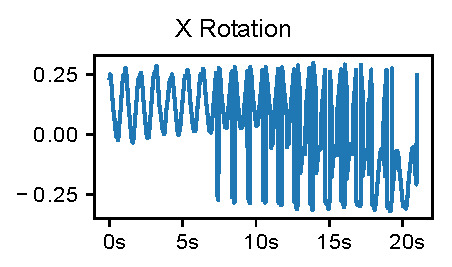
\includegraphics[width=\linewidth]{rotation_example.eps}
\caption{Examplary rotational sensor output recorded while walking.}
\label{myfig:rotation_sensor}
\end{figure}
Using the acceleration sensor without gravity is also a bad idea as this leads to an information loss. If the user has his phone in his pocket while sitting, gravity can be observed on the Z axis. In contrast it will be on the X axis, while he is standing.

This leads to the conclusion, that just using the acceleration sensor which includes gravity will lead to features which are easier to handle.

\section{Feature Selection and Windowing}
\label{sec:features}
The next task of this laboratory was to record measurements using the phone, transfer this measurements to a computer and define features which can later on be used in a \gls{knn} algorithm. To achieve this every class of activity was recorded four times. Three of these recordings were used for training and one to test classification using different features and ways of calculating them. In a first try the following features were calculated per test file:
\begin{itemize}
\item minimum of x acceleration
\item minimum of y acceleration
\item minimum of z acceleration
\item maximum of x acceleration
\item maximum of y acceleration
\item maximum of z acceleration
\item mean of x acceleration
\item mean of y acceleration
\item mean of z acceleration
\item standard deviation of x acceleration
\item standard deviation of y acceleration
\item standard deviation of z acceleration
\end{itemize}
This sums up to feature vectors whith a size of 12. For the \gls{knn} algorithm this means that three test files times six classes lead to a total of 18 samples. For the easier to detect classes like sitting and standing, this is already enough to work reliably. Classes which are harder to separate need a windowing approach which can be seen by comparing \fref{myfig:jogging_unwindowed} to \fref{myfig:jogging_windowed}.
\begin{figure}[htpb]
\centering
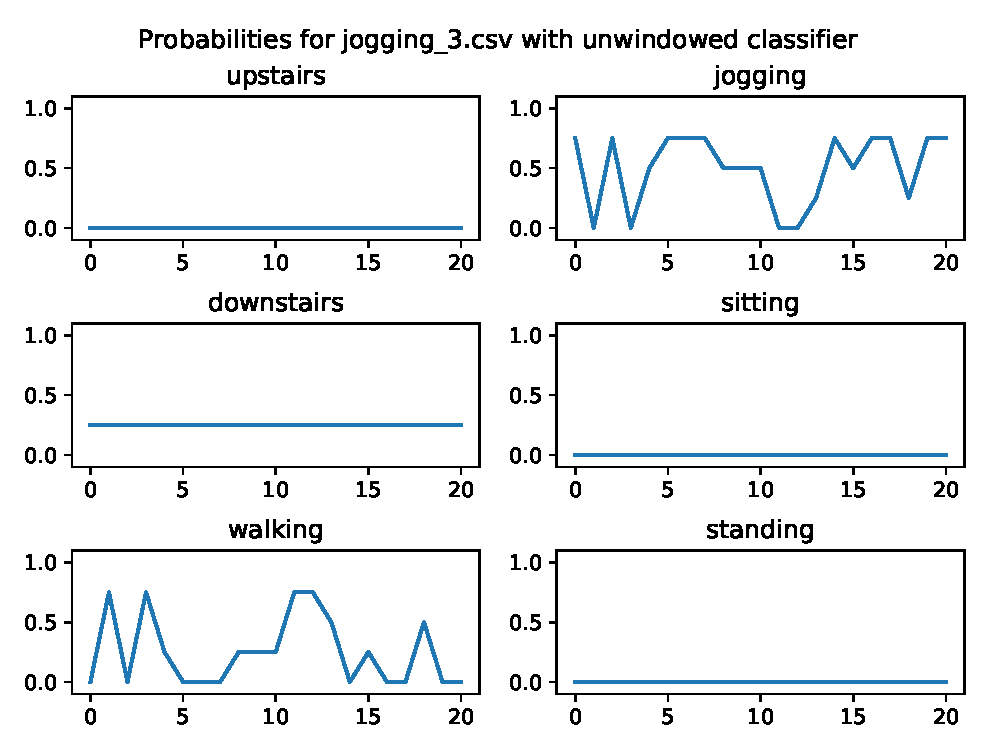
\includegraphics[width=\linewidth]{jogging_unwindowed.eps}
\caption{Classification with features generated without windowing.}
\label{myfig:jogging_unwindowed}
\end{figure}
\begin{figure}[htpb]
\centering
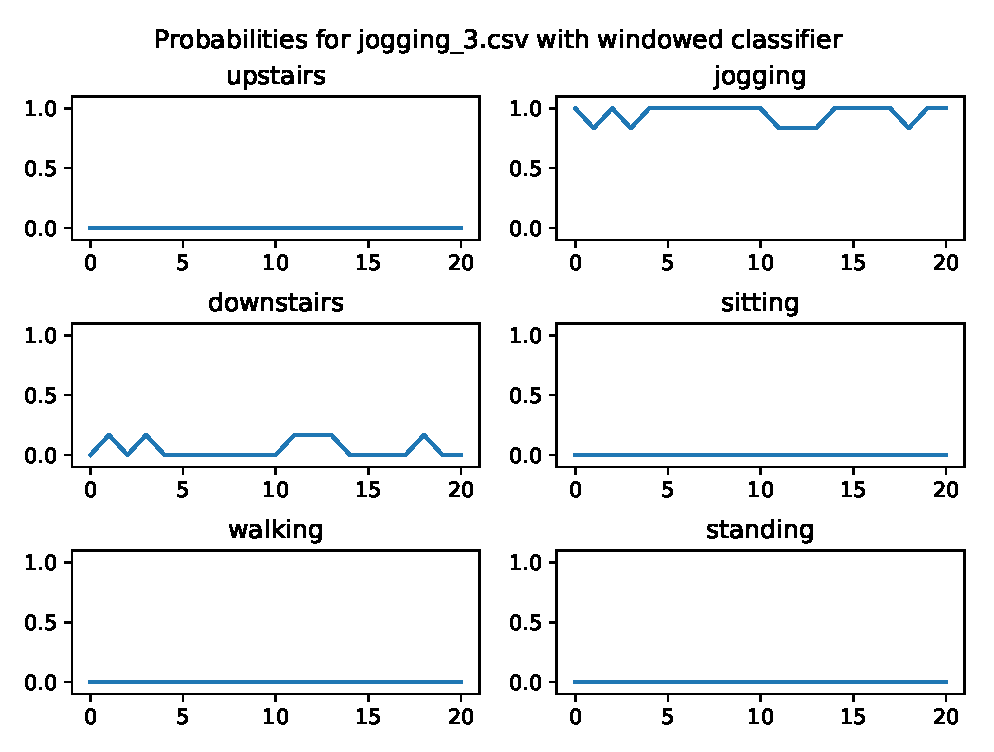
\includegraphics[width=\linewidth]{jogging_windowed.eps}
\caption{Classification with features generated with windowing.}
\label{myfig:jogging_windowed}
\end{figure}
Windowing was implemented by calculating one feature every \SI{1.2}{\second} over all files. To avoid the bias introduced by longer recordings leading to more features, the minimum amout available in all classes was chosen as a limit. The remaining feature vectors were discarded.

\section{Evaluating the KNN algorithm}
\label{sec:resultsKNN}
In the end of the first part of the laboratory, the \gls{knn} algorithm had to be implemented on the smartphone making use of the features precalculated on the computer. A video was recorded to demonstrate that the application is working. The recording was produced making use of the application \texttt{OBS-Studio}\autocite{obsproject:website}, as it is capable of mixing multiple streams. In detail, the screen of the smartphone as well as a camera stream of the recording device were used as sources.

\fref{myfig:knn_screenshot} shows one frame of the video. This frame shows the probabilities calculated by the \gls{knn} algorithm on the smartphone over time while the author of this report is jogging.
\begin{figure}[htpb]
\centering
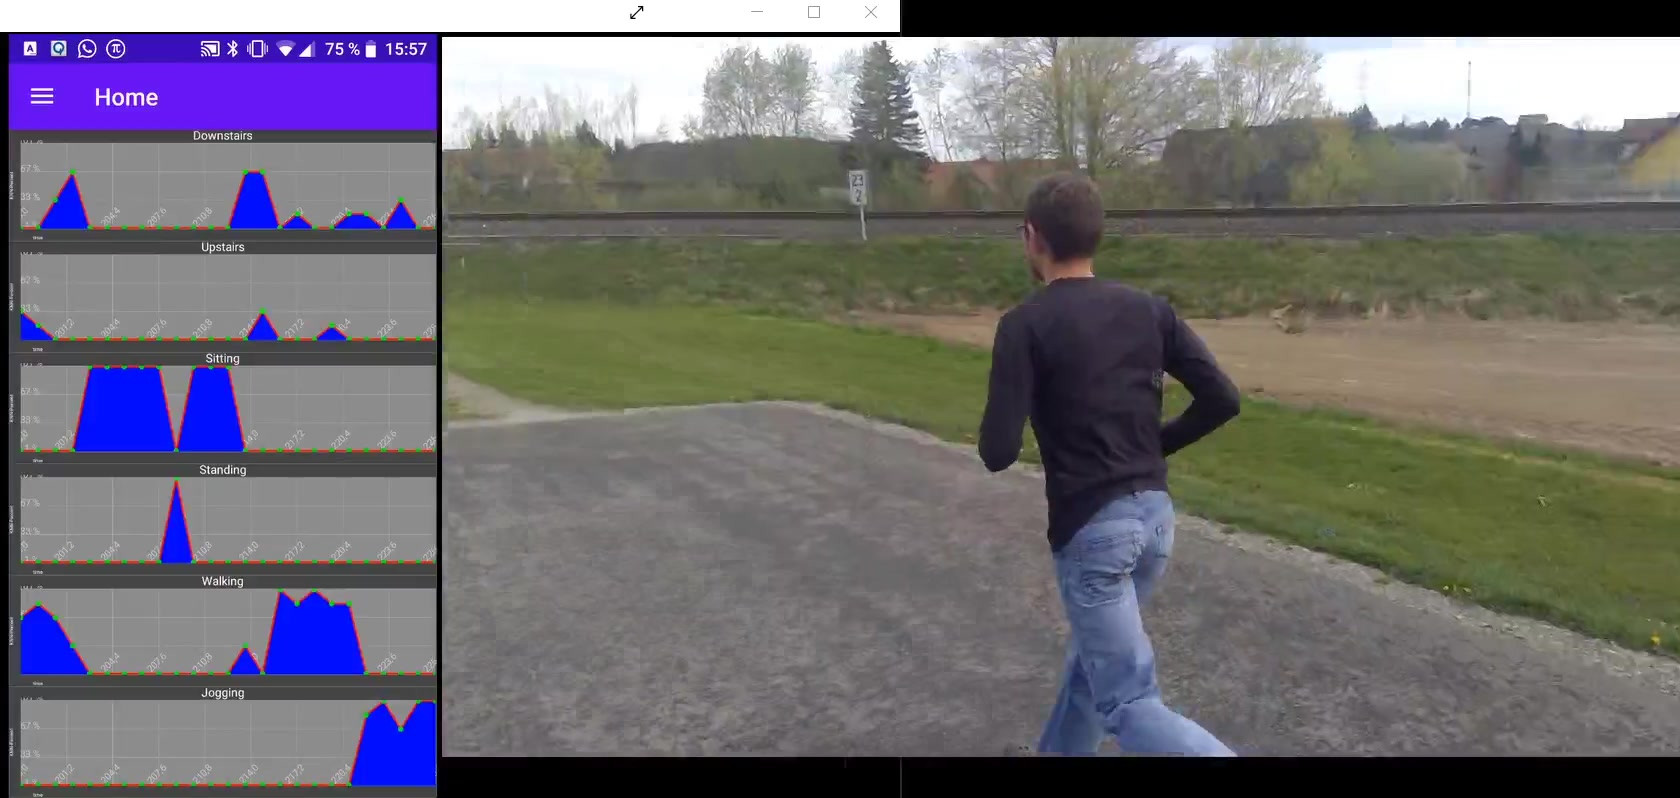
\includegraphics[width=\linewidth]{knn_screenshot}
\caption{One frame of the proof video demonstrating the \gls{knn} algorithm in action. The graph at the bottom depicts the probability of jogging.}
\label{myfig:knn_screenshot}
\end{figure}

\section{Developing a Base Model}
\label{sec:baseModel}
The course organization introduced the students of this laboratory to machine learning approaches by showing them how to train a model using the publicly available WISDM dataset\autocite{wisdm:dataset}. Performance of the provided example code is depicted for comparison in \fref{myfig:PlainGithub}.
\begin{figure}[htpb]
\centering
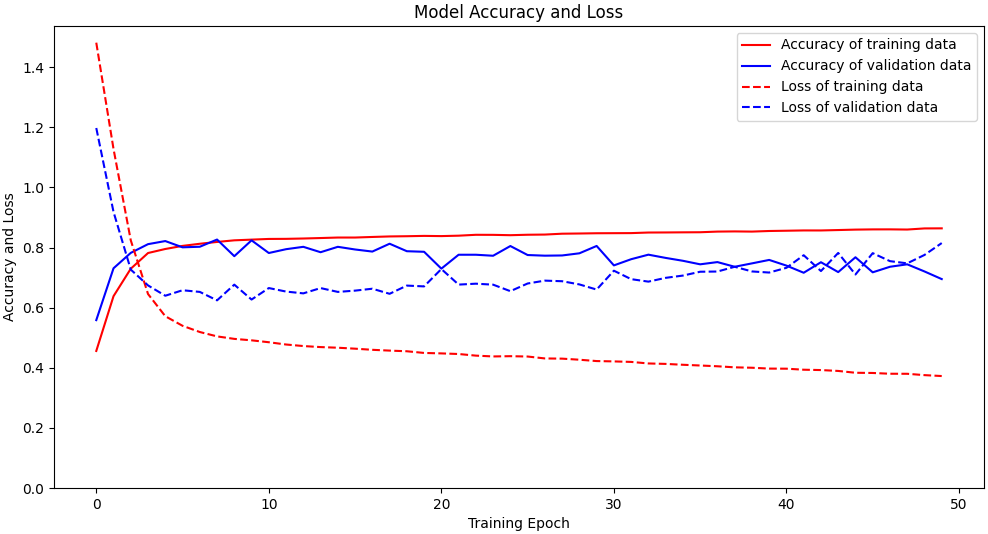
\includegraphics[width=\linewidth]{PlainGithub}
\caption{Performance of the base model example code provided by the course organziation.}
\label{myfig:PlainGithub}
\end{figure}
From this starting point a lot of optimizations were tried.

The first idea was to normalize the raw acceleration data in a different way than in the example code, as better normalized input data leads to faster convergence of machine learning models\autocite{Medium:Normalization}. The results shown in \fref{myfig:StdScaler} were generated using the \texttt{StandardScaler} module of \texttt{scikit-learn}\autocite{scikit:learn}.
\begin{figure}[htpb]
\centering
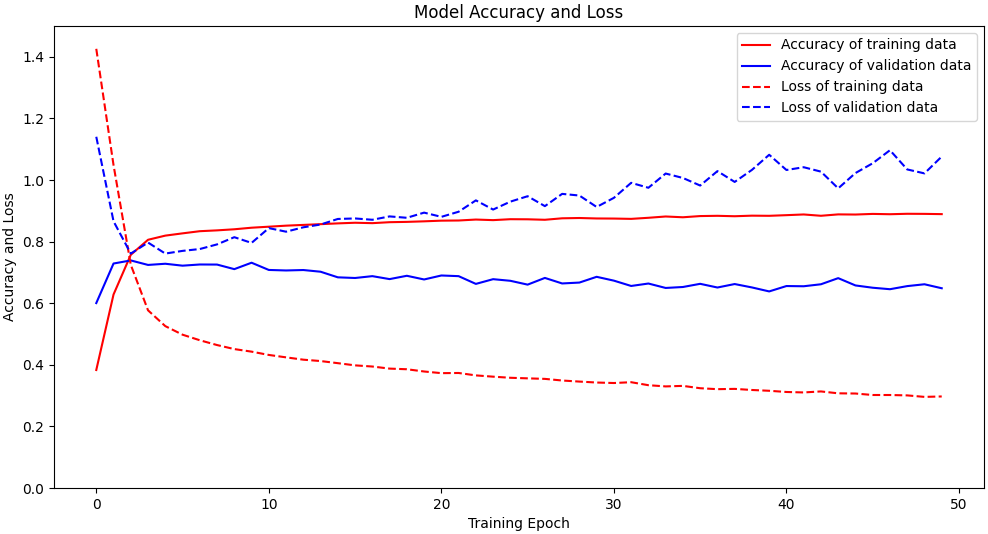
\includegraphics[width=\linewidth]{StdScaler}
\caption{Performance of the base model with better normalized input data using \texttt{StandardScaler} of \texttt{scikit-learn}.}
\label{myfig:StdScaler}
\end{figure}
Unfortunately the validation accuracy using this method performed slightly worse than the one of the given solution and the validation loss also increased.

The second idea was to split the training data by activities. The code given by the course organization just windows over all training data and assigns it with the label of the majority of samples. As depicted in \fref{myfig:SplitActivity}, implementing this change made it impossible for the network to converge.
\begin{figure}[htpb]
\centering
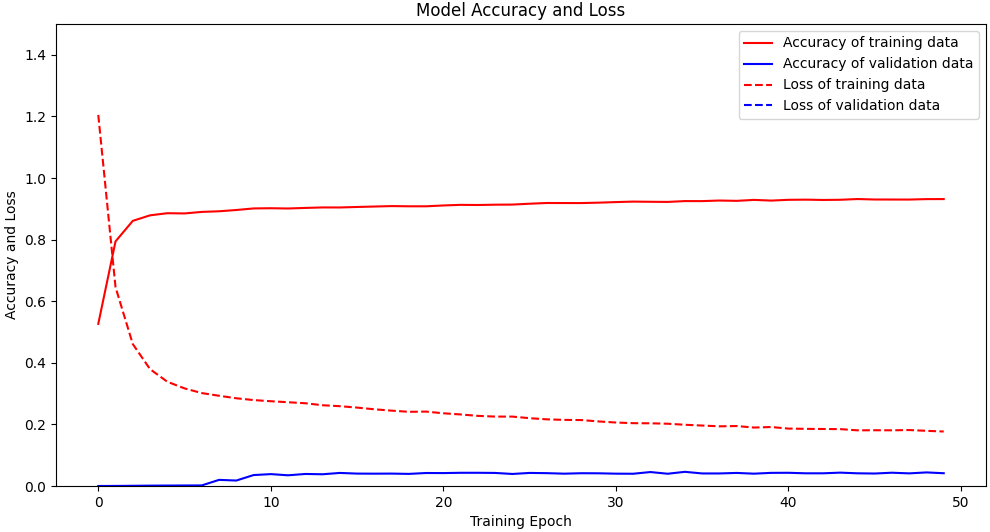
\includegraphics[width=\linewidth]{SplitActivity}
\caption{Performance of the base model with input data split by activities before windowing and labelling.}
\label{myfig:SplitActivity}
\end{figure}

The third approach was to change the network structure from just a combination of dense layers to:
\begin{enumerate}
\item convolutional layer with a height of 64
\item dropout layer with \SI{20}{\percent}
\item convolutional layer with a height of 32
\item dropout layer with \SI{20}{\percent}
\item convolutional layer with a height of 6
\item global average pooling layer
\item dense layer with softmax activation
\end{enumerate}
Note that the last convolutional layer results in a data cube with the 6 output classes as height. The global average pooling layer makes this convolutional layer learn the required pattern for identifying these classes. This approach was inspired by Martin Görner\autocite{Google:withoutPHD}. It results in much less computational effort than finishing convolutional layers with one or more dense layers. The performance of this model during training is depicted in \fref{myfig:DidiConvFinal}.
\begin{figure}[htpb]
\centering
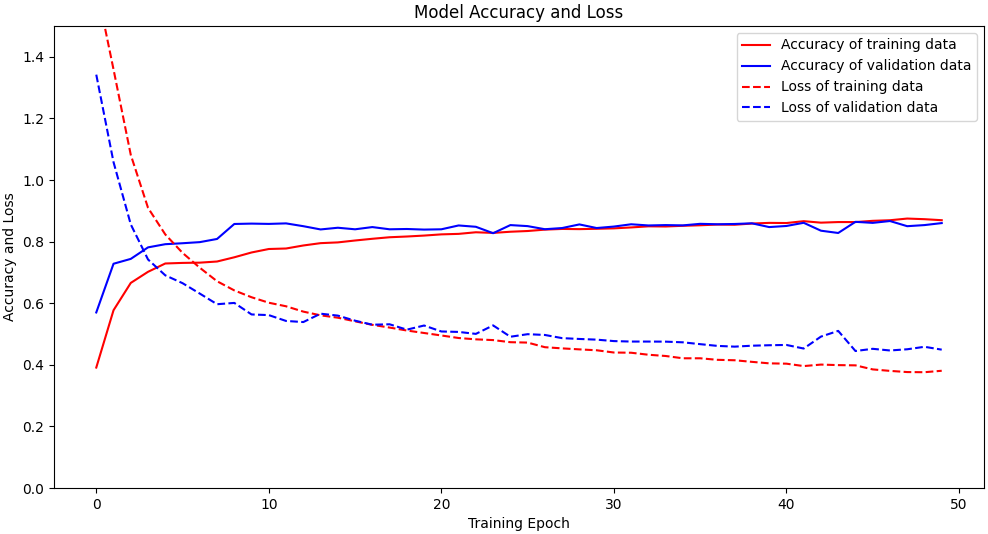
\includegraphics[width=\linewidth]{DidiConvFinal}
\caption{Performance of the base model with convolutional layers.}
\label{myfig:DidiConvFinal}
\end{figure}

In the end the improved base model's performance was measured using test data which was not shown to it during training or validation. The performance of the authors final model on this test data is depicted in \fref{myfig:DidiConvFinalConfusion} and can be compared to the model provided by the course organization in \fref{myfig:GithubConfusion}.
\begin{figure}[htpb]
\centering
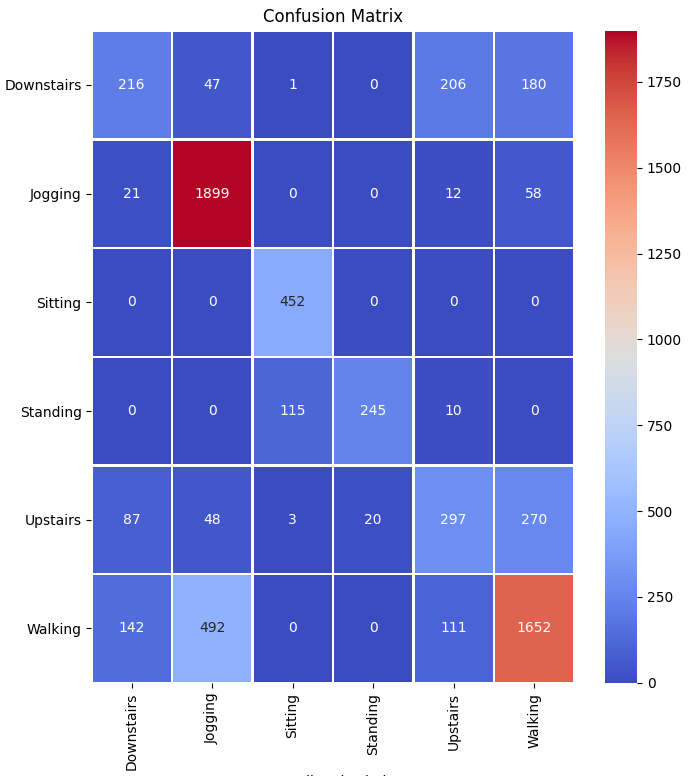
\includegraphics[width=\linewidth]{GithubConfusion}
\caption{Confusion matrix showing the performance of the model provided by the course organization.}
\label{myfig:GithubConfusion}
\end{figure}
\begin{figure}[htpb]
\centering
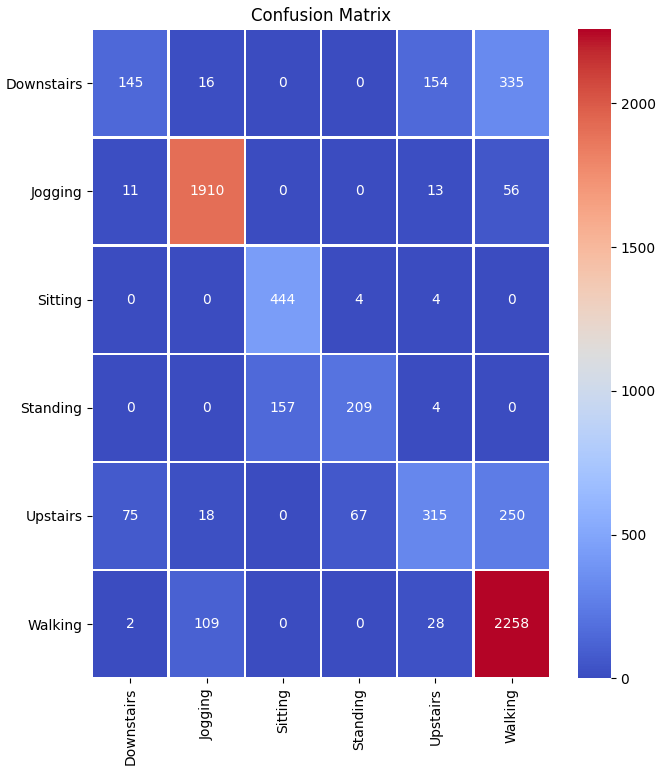
\includegraphics[width=\linewidth]{DidiConvFinalConfusion}
\caption{Confusion matrix showing the performance of the model by the author.}
\label{myfig:DidiConvFinalConfusion}
\end{figure}
Accuracy and loss values are compared in \fref{tab:accLoss}.
\begin{table}
\centering
\begin{tabular}[htpb]{rcc}
                    & Accuracy & Loss \\
Course Organization & 0.72 & 1.13 \\
Author              & 0.77 & 0.57 \\
\end{tabular}
\caption{Performance of the authors model compared to the model given by the course organization.}
\label{tab:accLoss}
\end{table}

%\FloatBarrier
\section{Creating the Head Model}
\label{sec:headModel}
For transfer learning a pre-trained base model is cut at a certain layer and new untrained layers are appended to it. These layers are trained directly on the target device. The code to do so was initially developed by Aaqib Saeed\autocite{saeed:transferLearning} as an example which is able to identify two separate classes. It was extended to the six classes described in \fref{sec:intro} and adapted to the base model developed in \fref{sec:baseModel}.

\section{Android Implementation}
\label{sec:android}
Most of the code for implementing transfer learning and running \texttt{TensorFlow} models on an android device was already developed by Aaqib Saeed\autocite{saeed:transferLearning} and the \texttt{TensorfFlow Lite} framework. The \gls{gui} was implemented from scratch and plots the prediction results of the \gls{knn} algorithm, the base model and the transfer learning model over time.
A settings frame which is shown in \fref{myfig:settings} of the app makes it possible to tell it the current position of the smartphone on the users body.
\begin{figure}[htpb]
\centering
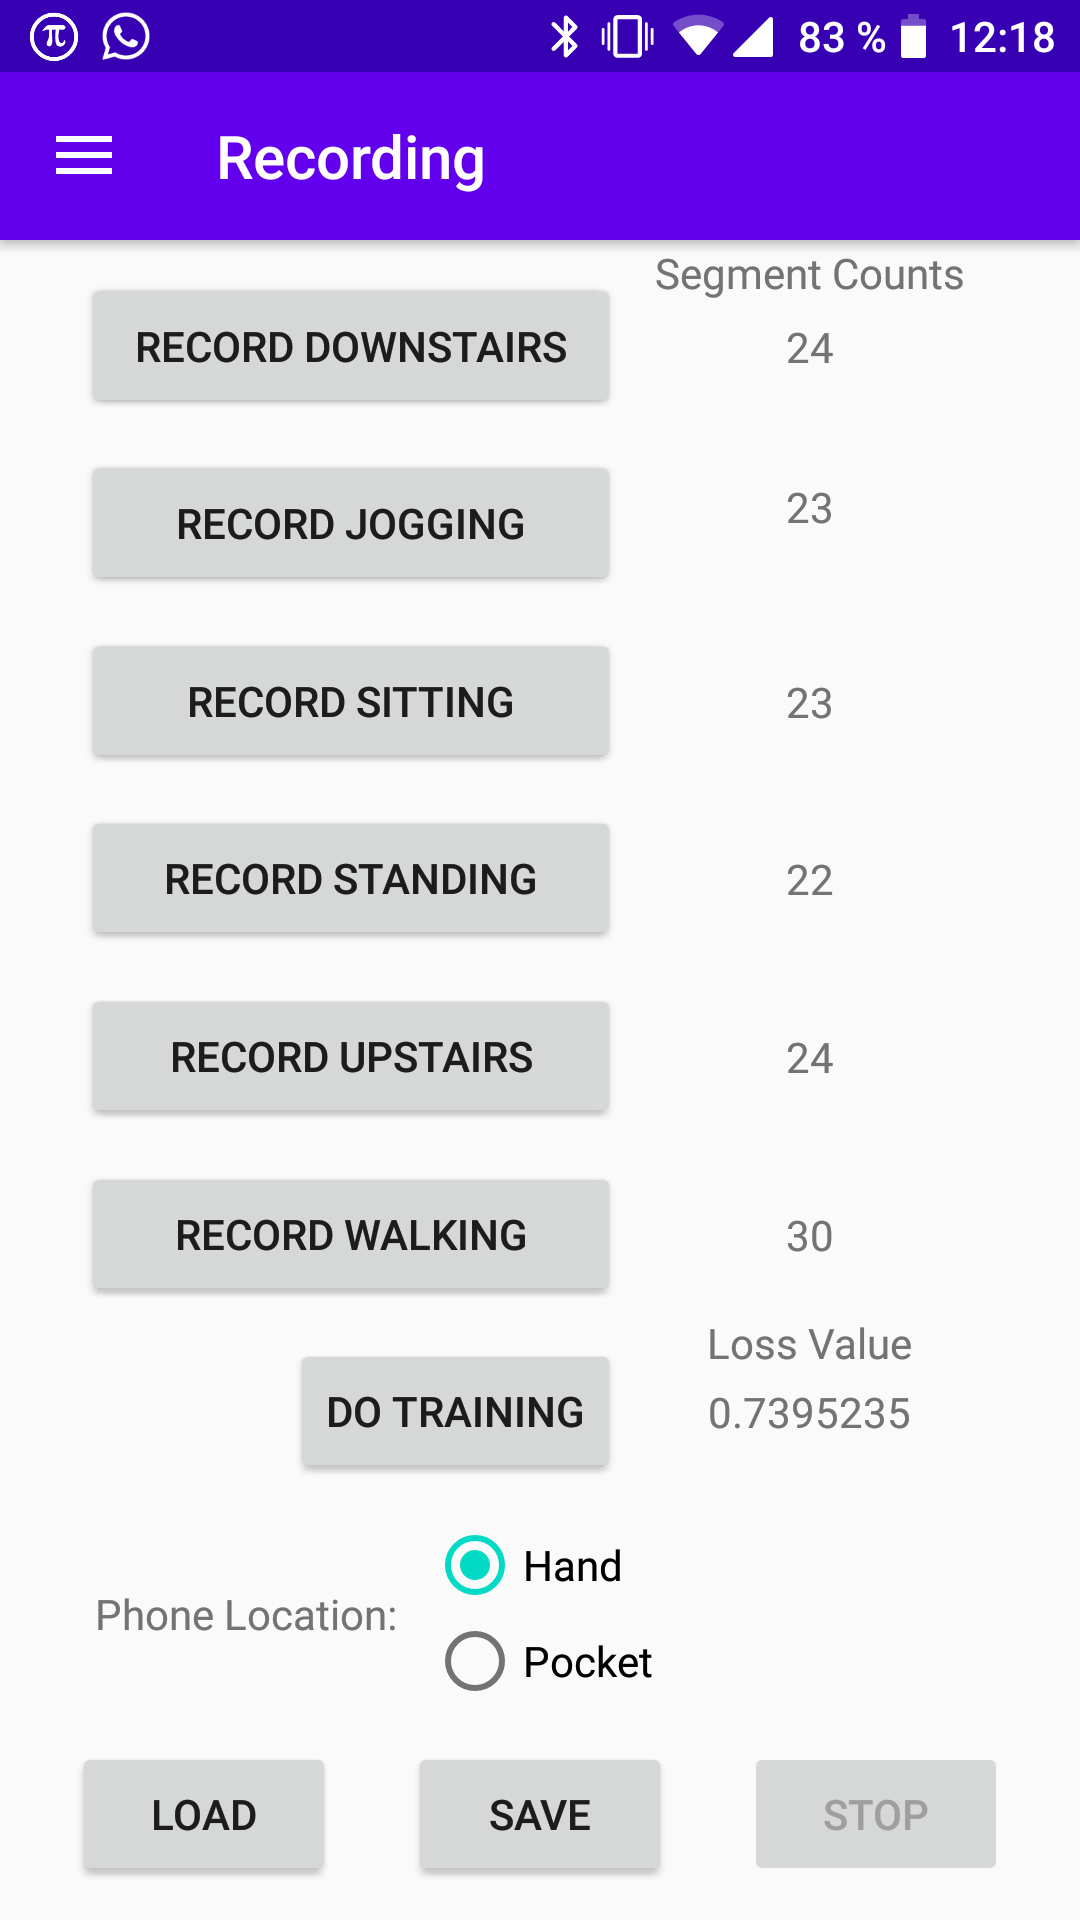
\includegraphics[width=\linewidth]{settingsFrame}
\caption{Screenshot of the settings frame of the android application.}
\label{myfig:settings}
\end{figure}

\section{Evaluating Machine Learning approaches}
\label{sec:resultsML}
The final goal of this laboratory was to compare classification results of the \gls{knn} algorithm with the base model and the transfer learning model. This was again done using a video recording as described in \fref{sec:resultsKNN}.

\fref{myfig:all_screenshot} shows one frame of this recording in which the author of this report is standing. \gls{knn} as well as the transfer learning model would correctly classify standing, as the smartphone is lieing in an angle similar to being in the pocket where the \gls{knn} measurements were taken. Unfortunately the base model thinks the user is going upstairs.
\begin{figure}[htpb]
\centering
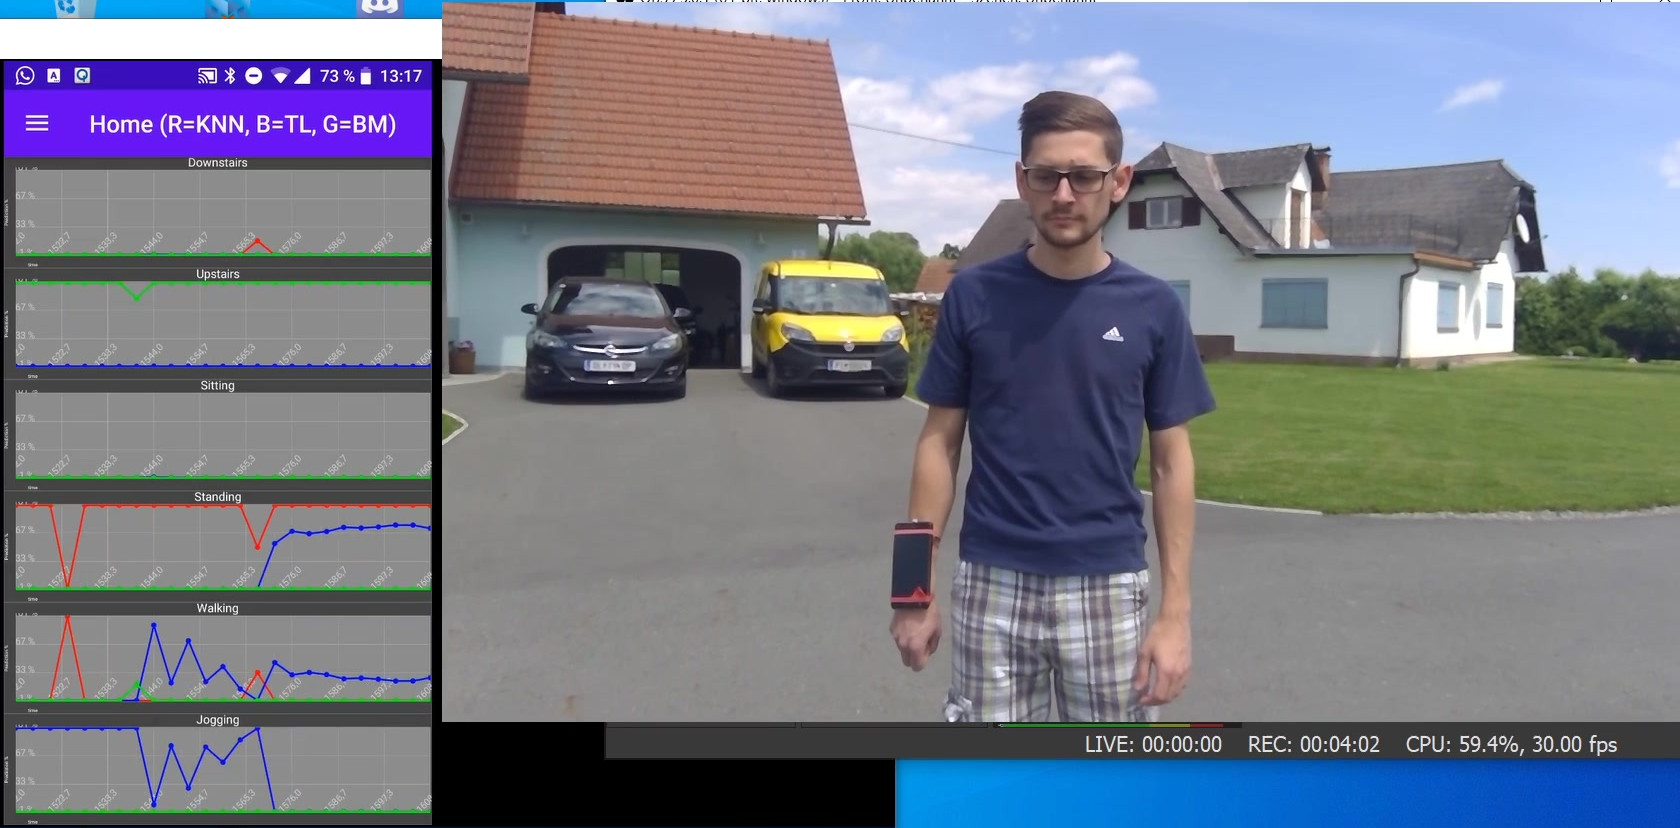
\includegraphics[width=\linewidth]{all_screenshot}
\caption{One frame of the proof video demonstrating the comparison of all implemented algorithms.}
\label{myfig:all_screenshot}
\end{figure}

\fref{myfig:sitting} shows a screenshot which was taken while the user was sitting with the phone in its pocket. This situation also displays, that \gls{knn} and the transfer learning model trained to this location of the phone are working. In contrast \fref{myfig:knn_wrong_screenshot} shows a screenshot which was taken while the user is walking and has the phone attached to its hand like in \fref{myfig:all_screenshot}. In this situation the \gls{knn} algorithm performs worse, because it was trained with the phone in the pocket. The transfer learning model was trained on device with the phone attached to the users hand. This is why it is able to correctly classify walking in this situation.
\begin{figure}[htpb]
\centering
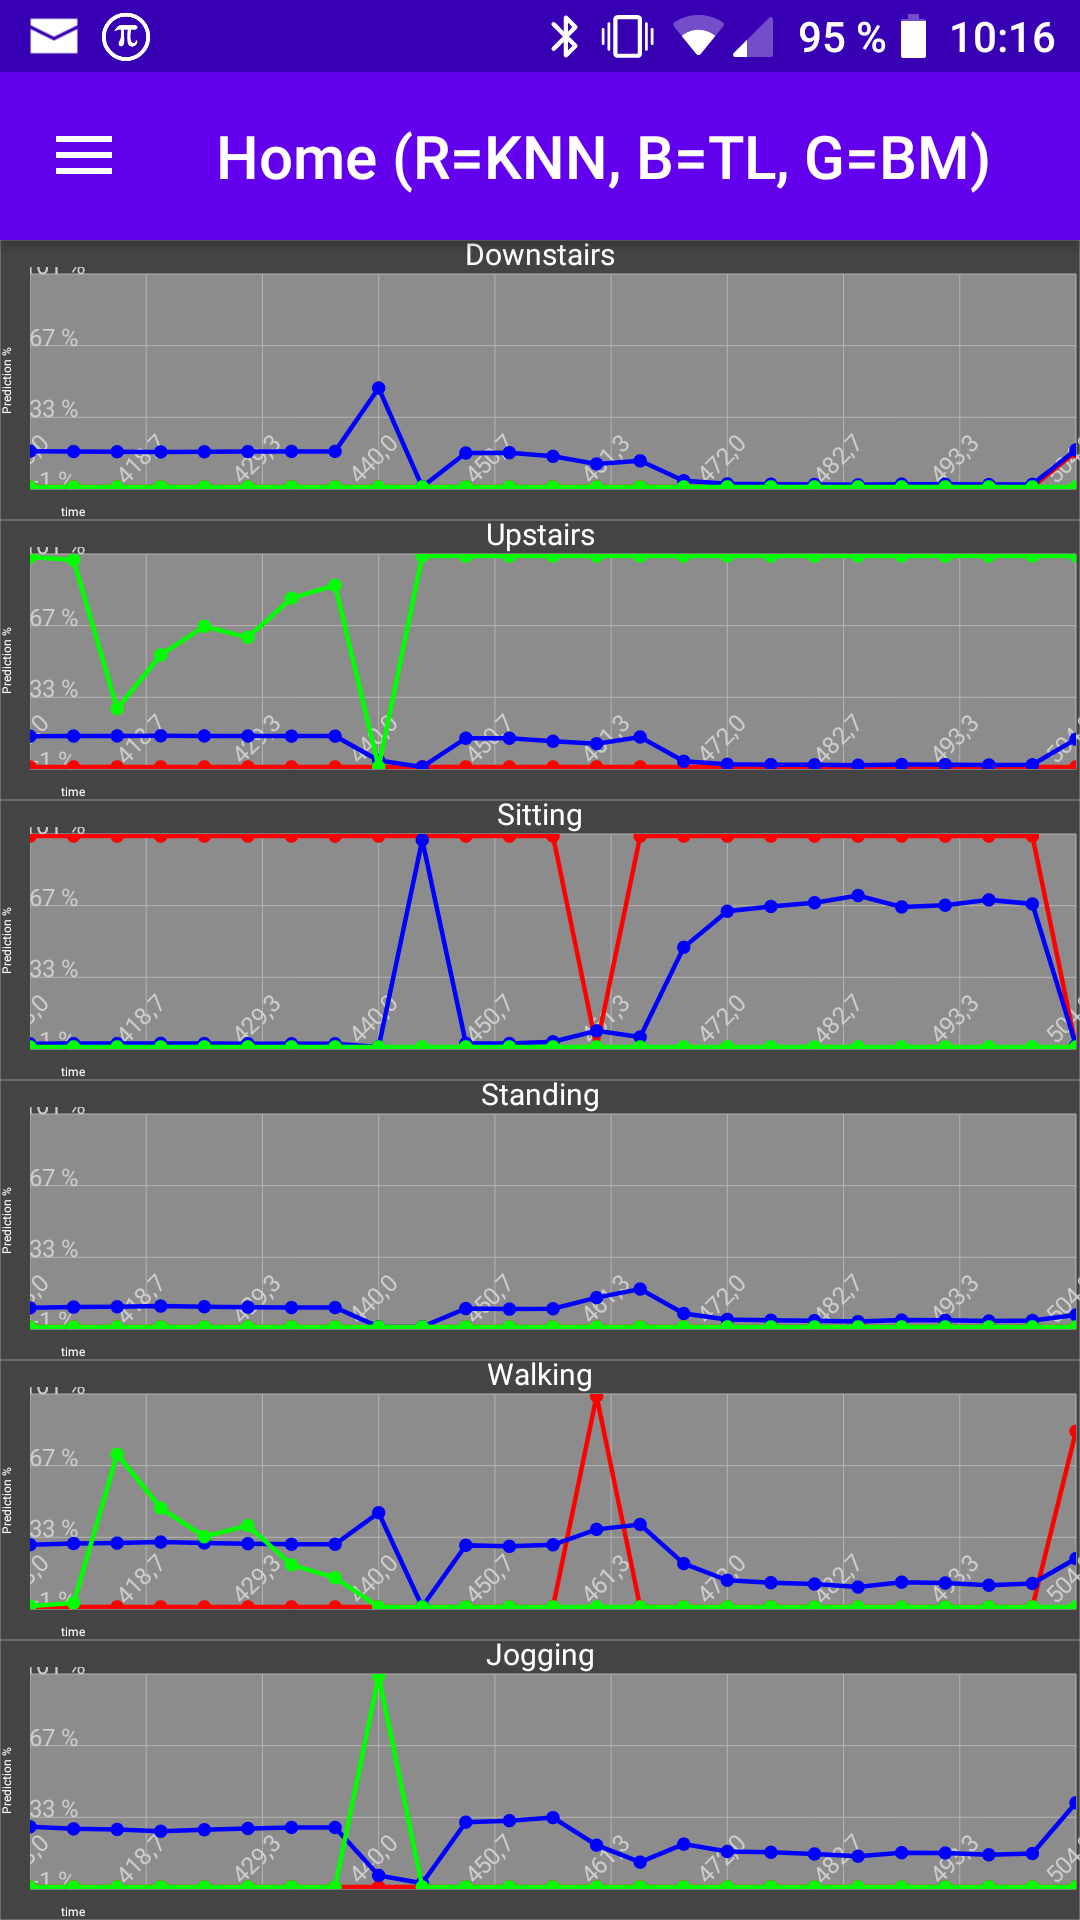
\includegraphics[width=\linewidth]{sitting}
\caption{Screenshot of the application taken while the user was sitting with the phone in its pocket.}
\label{myfig:sitting}
\end{figure}
\begin{figure}[htpb]
\centering
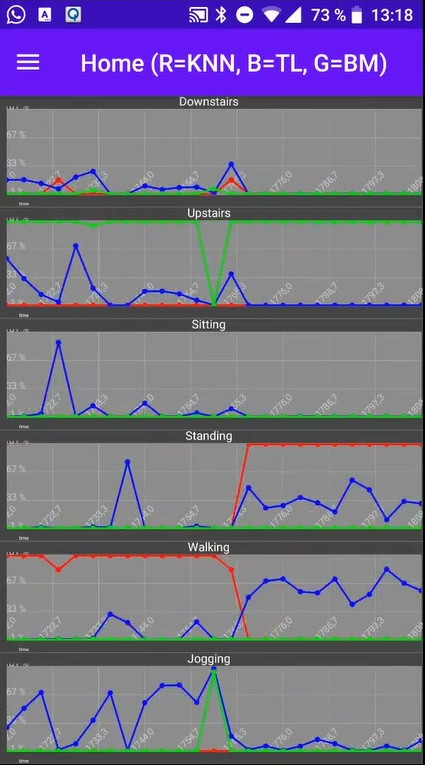
\includegraphics[width=\linewidth]{knn_wrong_screenshot}
\caption{Screenshot of the application taken while the user was walking with the phone attached to its hand.}
\label{myfig:knn_wrong_screenshot}
\end{figure}

To have a quantitative estimation of the apps performance, a logging functionality was implemented in the end. This made it possible to record classification results of all three methods into a file. One file per class and smartphone position was recorded and later on evaluated on a PC. This led to the results depicted in \fref{tab:classPerf}.
\begin{table}
\centering
\begin{tabular}[htpb]{rSSS}
                             & {KNN} & {TL} & {BM} \\
downstairs, phone on hand & 0.0 & 65.5 & 0.0 \\
jogging, phone on hand & 0.0 & 34.6 & 88.8 \\
sitting, phone on hand & 0.0 & 0.0 & 0.0 \\
standing, phone on hand & 100.0 & 62.4 & 0.0 \\
upstairs, phone on hand & 0.0 & 39.2 & 0.0 \\
walking, phone on hand & 0.0 & 28.5 & 0.0 \\
downstairs, phone in pocket & 34.7 & 0.0 & 0.0 \\
jogging, phone in pocket & 12.0 & 41.1 & 94.1 \\
sitting, phone in pocket & 100.0 & 100.0 & 0.0 \\
standing, phone in pocket & 100.0 & 0.0 & 0.0 \\
upstairs, phone in pocket & 0.0 & 0.0 & 0.0 \\
walking, phone in pocket & 88.0 & 100.0 & 0.0 \\
\end{tabular}
\caption{Classification performance of all three algorithms in percent.}
\label{tab:classPerf}
\end{table}
\section{Conclusion}
As shown in \fref{sec:resultsML}, the \gls{knn} classifier worked better than expected as long as the phone is at the position at which it was during the initial recordings. The base model pre trained by the WISDM dataset did not provide good results in this case. The transfer learning based approach made it possible to train the neuronal network to a new smartphone position directly on the device.

% if have a single appendix:
%\appendix[Proof of the Zonklar Equations]
% or
%\appendix  % for no appendix heading
% do not use \section anymore after \appendix, only \section*
% is possibly needed

% use \appendices with more than one appendix
% then use \section to start each appendix
% you must declare a \section before using any
% \subsection or using \label (\appendices by itself
% starts a section numbered zero.)
%
% you can choose not to have a title for an appendix
% if you want by leaving the argument blank
%\appendix
%\section{}
%Appendix two text goes here.

\appendix[Development Repository]
\label{sec:appendix}
All data created during this laboratory was initially versioned at \url{https://git.tugraz.at/MobileComputingLab.git} using the credentials provided to the system at \url{https://git.tugraz.at/} to prevent plagiarism blames. It is now publicly available at \url{https://github.com/didi1357}.


% use section* for acknowledgment
\section*{Acknowledgment}
The author would like to thank the whole Mobile Computing Laboratory team for their time and dedication.

% Can use something like this to put references on a page
% by themselves when using endfloat and the captionsoff option.
\ifCLASSOPTIONcaptionsoff
  \newpage
\fi


% trigger a \newpage just before the given reference
% number - used to balance the columns on the last page
% adjust value as needed - may need to be readjusted if
% the document is modified later
%\IEEEtriggeratref{8}
% The "triggered" command can be changed if desired:
%\IEEEtriggercmd{\enlargethispage{-5in}}

\printbibliography

% biography section
% 
% If you have an EPS/PDF photo (graphicx package needed) extra braces are
% needed around the contents of the optional argument to biography to prevent
% the LaTeX parser from getting confused when it sees the complicated
% \includegraphics command within an optional argument. (You could create
% your own custom macro containing the \includegraphics command to make things
% simpler here.)
%\begin{IEEEbiography}[{\includegraphics[width=1in,height=1.25in,clip,keepaspectratio]{mshell}}]{Michael Shell}
% or if you just want to reserve a space for a photo:

\vfill

\begin{IEEEbiography}[{\includegraphics[width=1in,height=1.25in,clip,keepaspectratio]{malli}}]{Dietmar Malli}%
was born in Deutschlandsberg, Styria, Austria in 1995. He went to local schools there and is working for the company mse elektronik GmbH in Graz since 2012. Currently he is studying Information and Computer Engineering at the Technical University Graz where he also earned a Bachelor's degree in this program of study.
\end{IEEEbiography}

% if you will not have a photo at all:
%\begin{IEEEbiographynophoto}{John Doe}
%Biography text here.
%\end{IEEEbiographynophoto}

% insert where needed to balance the two columns on the last page with
% biographies
%\newpage

%\begin{IEEEbiographynophoto}{Jane Doe}
%Biography text here.
%\end{IEEEbiographynophoto}

% You can push biographies down or up by placing
% a \vfill before or after them. The appropriate
% use of \vfill depends on what kind of text is
% on the last page and whether or not the columns
% are being equalized.

% Can be used to pull up biographies so that the bottom of the last one
% is flush with the other column.
%\enlargethispage{-5in}



% that's all folks
\end{document}


